\documentclass{article}
\usepackage{amsmath}
\usepackage{amssymb}
\usepackage{graphicx}
\usepackage{hyperref}
\usepackage[version=4]{mhchem}


\begin{document}
\section*{Problem}
(2009 AIME) In parallelogram \(A B C D\), point \(M\) is on \(A B\) so that \(\frac{A M}{A B}=\frac{17}{1000}\), and point \(N\) is on \(A D\) so that \(\frac{A N}{A D}=\frac{17}{2009}\). Let \(P\) be the point of intersection of \(A C\) and \(M N\). Find \(\frac{A C}{A P}\).\\
\centering
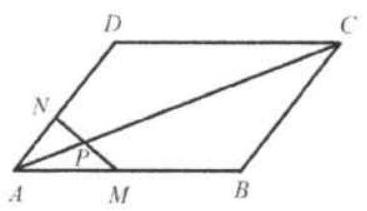
\includegraphics[width=\textwidth]{images/130(2).jpg}

\section*{Solution}
177.
Method 1:\\
Let point \(S\) be on \(A C\) such that \(N S\) is parallel to \(A B\).\\
Because \(\triangle A S N\) is similar to \(\triangle A C D, A S / A C=(A P+P S) / A C\) \(=A N / A D=17 / 2009\).\\
Because \(\triangle P S N\) is similar to \(\triangle P A M, P S / A P=S N / A M\)\\
\centering
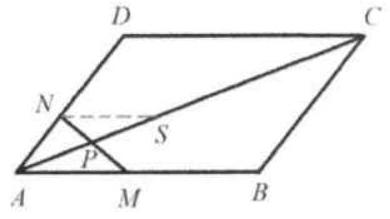
\includegraphics[width=\textwidth]{images/141(2).jpg}\\
\(=\frac{\frac{17}{2009} C D}{\frac{17}{1000} A B}=\frac{1000}{2009}\), and so \(\frac{P S}{A P}+1=\frac{3009}{2009}\).\\
Hence \(\frac{\frac{17}{2009} A C}{A P}=\frac{3009}{2009}\), and \(\frac{A C}{A P}=177\).\\
Method 2:\\
Extend \(N M\) through \(M\) to \(E\) and to meet the extension of \(C B\) at \(E\).


We label the line segments as shown in the figure 1. We know that \(A D / / C E\). So \(\triangle A M N \sim \triangle B M E\) (Figure 1).\\
\(\frac{A N}{B E}=\frac{A M}{M B} \Rightarrow \quad \frac{17 y}{B E}=\frac{17 x}{983 x} \Rightarrow B E=983 y\).\\
We know that \(A N / / C E\). So \(\triangle A P N \sim \triangle C P E\) (Figure 2).\\
\centering
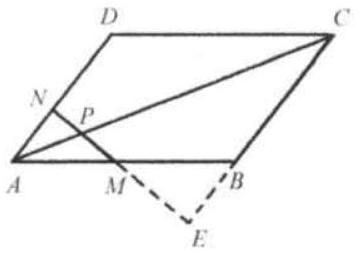
\includegraphics[width=\textwidth]{images/142(2).jpg}

\[
\begin{aligned}
& \frac{A N}{C E}=\frac{A P}{P C} \quad \Rightarrow \frac{17 y}{(2009+983) y}=\frac{A P}{A C-A P} \quad \Rightarrow \\
& \frac{A C}{A P}-1=\frac{2992}{17} \quad \Rightarrow \quad \frac{A C}{A P}=\frac{2992}{17}+1=177 .
\end{aligned}
\]

\begin{center}
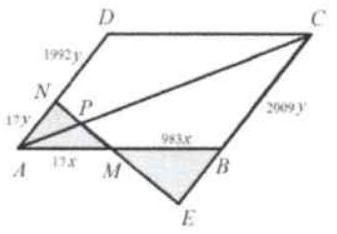
\includegraphics[width=\textwidth]{images/142(1).jpg}
\end{center}

Figure 1\\
\centering
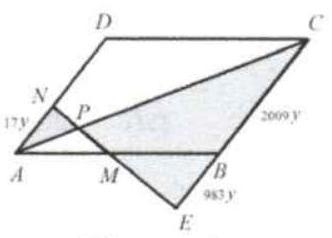
\includegraphics[width=\textwidth]{images/142(4).jpg}

Figure 2

\end{document}
